\draft Classic quantum Hall effect question.

\begin{parts}
	\part The quantum Hall effect is a phenomenon where the Hall resistivity $\rho_{xy}$ is quantised to take $\diagfrac{1}{n}$ where $n$ is an integer.
	This is attributed to the formation of Landau levels on large field limit where $\omega_c \tau \gg 1$ ($\omega_c = eB/m_{CR}$ is the cyclotron frequency, $\tau$ is the scattering time).

	\begin{figure}[H]
		\centering
		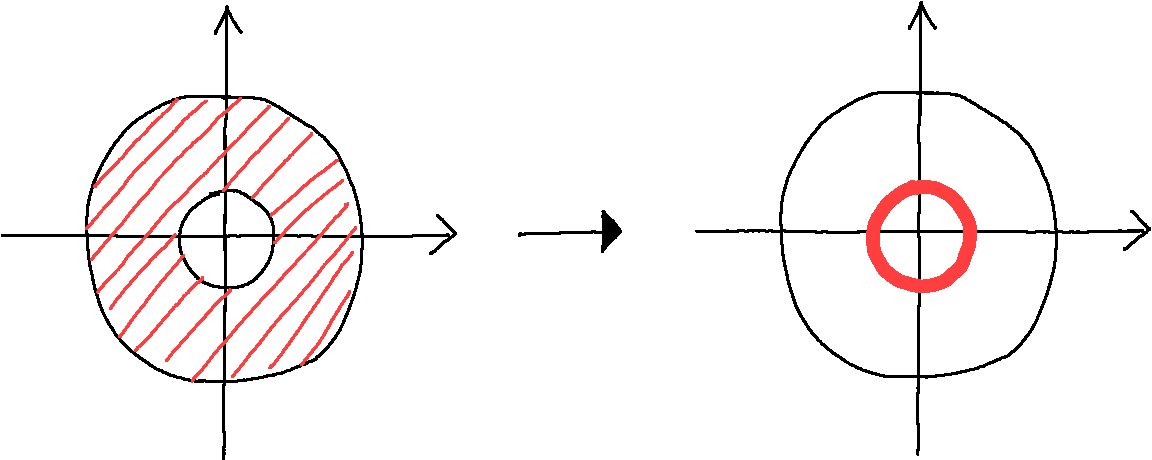
\includegraphics[width=.6\linewidth]{q6-landau-lvl}
	\end{figure}
	
	Introduction of Landau levels squeezes the free electron into each ring, so for each Landau ring we have areal density:
	\begin{align*}
		n_l &= \frac{1}{\rbracket{2\pi}^2} \cdot \pi \rbracket{k_{l+1}^2 - k_l^2} \\
		&= \frac{1}{4\pi} \cdot \frac{2m}{\hbar} \cdot \frac{eB}{m} \\
		&= \frac{eB}{h}
	\end{align*}
	
	Hence in total we have total areal density:
	\begin{align*}
		N_s &= n_l \cdot \nu \\
			&= \frac{eB\nu}{h} \mtext{where $\nu \in \mathcal{Z}$ is the filling factor}
	\end{align*}
	
	Note that for a changing $B$ we have a period of $\Delta(1/B) = e/hN_s$.
	And the reason why Hall resistivity may be used as a resistance standard is due to it purely being the ratio of fundamental constants $h$ and $e$.
	
	\part Sketch of setup:
	\begin{figure}[H]
		\centering
		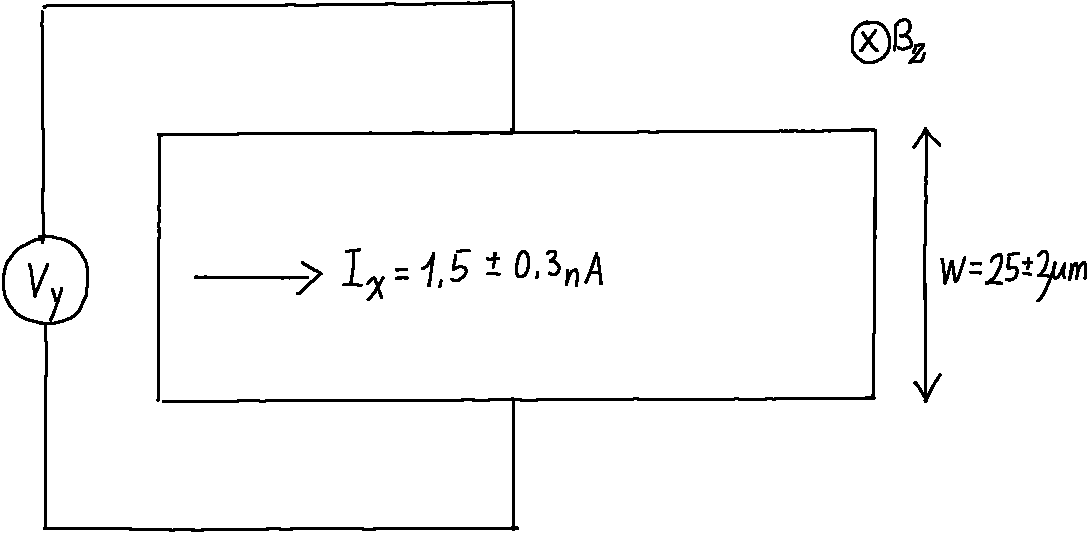
\includegraphics[width=.8\linewidth]{q6-expr-setup}
	\end{figure}
	
	From Drude:
	\begin{gather*}
		\deri{\mathbf{p}}{t} = q\rbracket{\mathbf{E} + \mathbf{v}\times\mathbf{B}} - \frac{\mathbf{p}}{\tau} \\
		\xRightarrow{\textnormal{Steady state}}d\mathbf{p}/dt = 0
	\end{gather*}
	\begin{numcases}{}
		v_x = \frac{q\tau}{m} \rbracket{E_x + v_y B_z} \label{eqn:q6-drude-x} \\
		v_y = \frac{q\tau}{m} \rbracket{E_y - v_x B_z} \label{eqn:q6-drude-y}
	\end{numcases}
	
	Enforcing the condition of no Hall current gives $v_y = 0$:
	\begin{align*}
		E_y &= v_x B_z \\
		\xRightarrow{\eqref{eqn:q6-drude-x}} E_y &= \frac{qB_z}{m}\tau E_x \\
		\frac{E_y}{E_x} &= \omega_c \tau
	\end{align*}
	
	Also resistivity in the limit $\omega_c \tau \gg 1$:
	\begin{align*}
		\rho_{yx} &= R_H B \\
		&= \frac{E_y}{J_x} \\
		&= \frac{E_y}{N_s q v_x} \\
		&= \frac{B_z}{N_s q} \\
		&= \frac{1}{\nu} \frac{h}{eB_z} \cdot \frac{B_z}{e} \\
		&= \frac{1}{\nu} \cdot \frac{h}{e^2}
	\end{align*}
	
	We also know that $V_y = E_y w$, $I_x = J_x w$:
	\begin{align*}
		\frac{V_y}{I_x} &= \rho_{yx} \\
		V_y &= I_x \rho_{yx} \\
		&= \frac{h}{\mu e^2}I_x \\
		&= \begin{cases}
			\SI{3.87e-4}{\volt} \qquad \nu = 1 \\
			\SI{1.94e-4}{\volt} \qquad \nu = 2 \\
			\SI{1.29e-4}{\volt} \qquad \nu = 3 \\
			\SI{9.68e-5}{\volt} \qquad \nu = 4
		\end{cases}
	\end{align*}
	
	Error analysis:
	\begin{equation*}
		\Delta\rbracket{\frac{V_y}{I_x}} = \textnormal{sum of \% errors} = \textnormal{2\% from $I_x$ ($w$ cancels)}
	\end{equation*}
	
	Assuming the top peak corresponds to $\nu = 1$, we then have:
	\begin{align*}
		\begin{aligned}
			19x &= \SI{3.87e-4}{\volt} \\
			12x &= \SI{1.94e-4}{\volt} \\
			9x &= \SI{1.29e-4}{\volt} \\
			6x &= \SI{9.68e-5}{\volt}
		\end{aligned}
		\qquad & \Rightarrow \qquad
		x = \begin{cases}
			\SI{2.04e-5}{\volt/unit} \\
			\SI{1.62e-5}{\volt/unit} \\
			\SI{1.43e-5}{\volt/unit} \\
			\SI{1.61e-5}{\volt/unit}
		\end{cases} \\
		&\Rightarrow \lambda \equiv \bar{x} = \SI{1.68e-5}{\volt/unit} \pm 2\%
	\end{align*}
	
	\part Sketch of $\rho_{xx}$ against $B$:
	\begin{figure}[H]
		\centering
		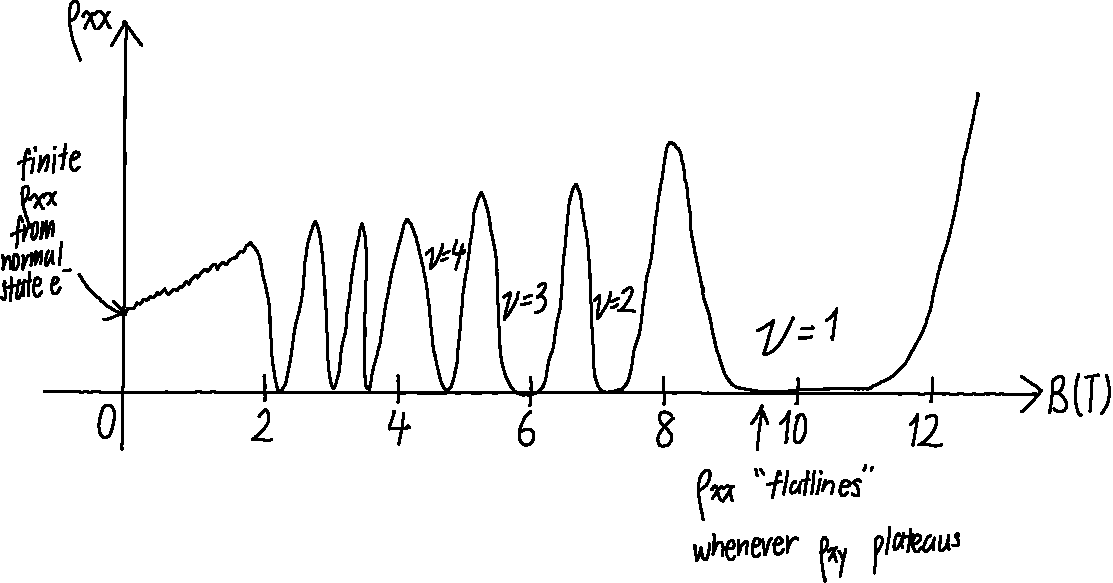
\includegraphics[width=.7\linewidth]{q6-rho-xx}
	\end{figure}
	
	Sketch of d.o.s.:
	\begin{figure}[H]
		\centering
		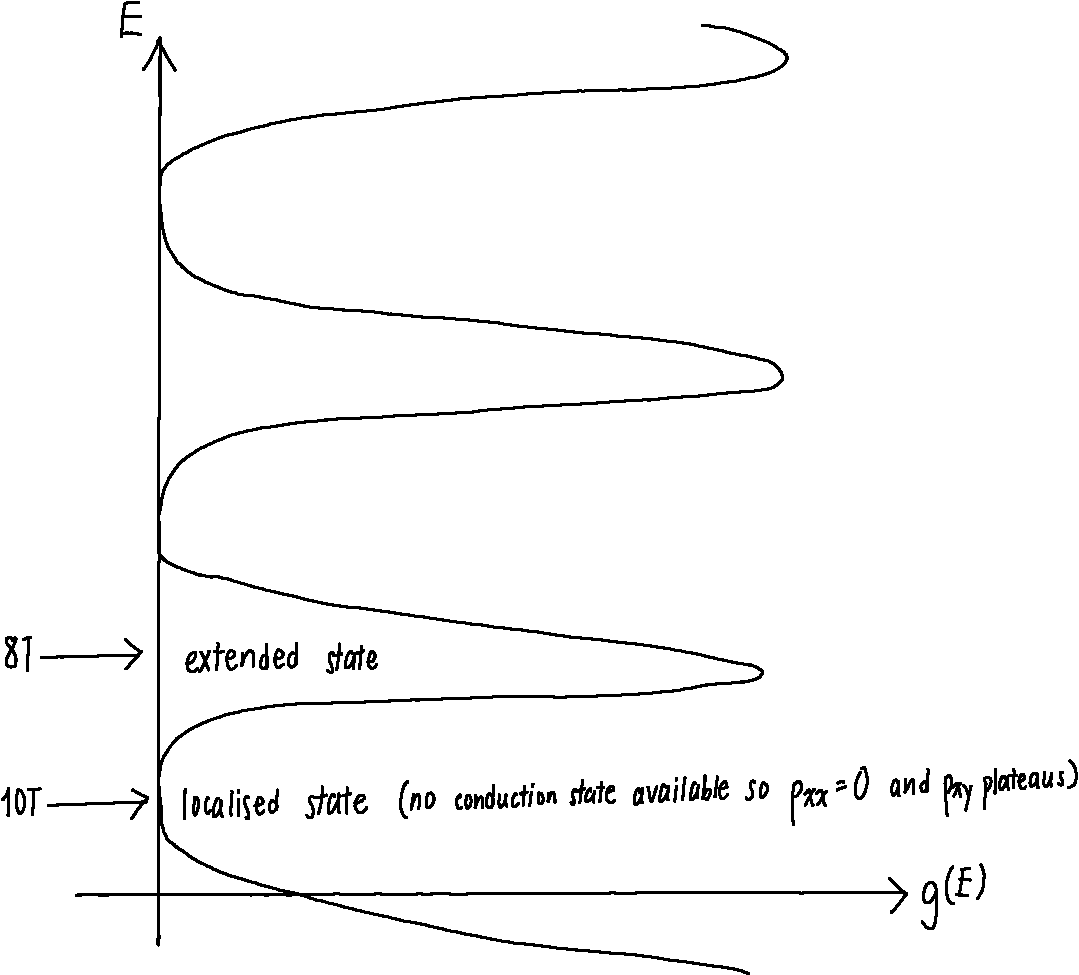
\includegraphics[width=.7\linewidth]{q6-dos}
	\end{figure}
	
	\part As $B_z$ increases, the filling factor decreases as each Landau level may accommodate more states.
	When $\nu$ is an integer, we have a fully filled Landau level which can contribute no longitudinal current $\Rightarrow$ fixed Hall voltage.
	
	The reason why we have a jump over some range of $B$ is due to the variation of Landau level throughout the sample due to impurities.
	This gives rise to localised states where electrons available for conduction are not globally connected, rendering $\rho_{xx} = 0$.
	And extended states where the opposite happens.
	
	\begin{figure}[H]
		\centering
		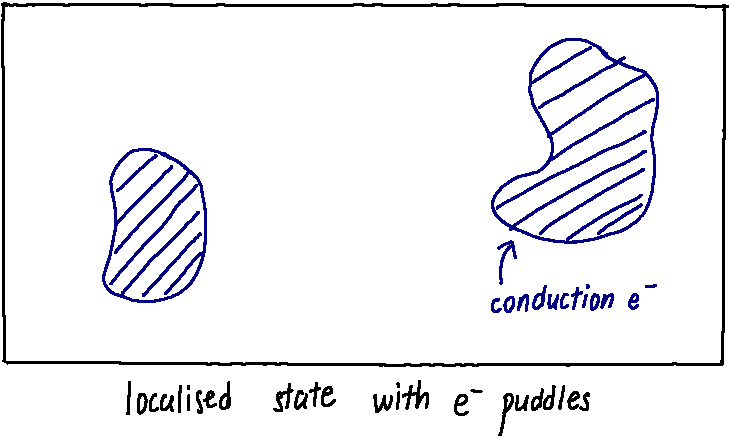
\includegraphics[width=.6\linewidth]{q6-localised-states}
	\end{figure}
\end{parts}